\chapter{Progress on the Open Problems}\label{chap:progress}

\Cref{chap:open} lists the questions this book leaves open. This chapter
reports what happened when we worked on six of them. Two move substantially.
The third cumulant of the stopping time (O4), the last unexplained statistic in
\cref{chap:stochastic}, turns out to behave exactly like the variance: its
deficit against the Bernoulli model behaves, up to $2^{49}$, as an additive constant located mostly in the
final descent of the orbit, and a two parameter fit from the census predicts
the skewness of stopping times out of sample, at starting values $2^{19}$ times
larger, to within two standard errors. And the exact convex rate of Switching
MM (P11) now has a complete conjectured closed form, with two branches and
exact thresholds, rigorous lower bounds from explicit functions, and a proof
of the upper bound for two and four steps, for $\beta$ up to $0.6446$ and $0.7043$, by an explicit certificate. Four
more problems advance by computation: the noise theory of \cref{chap:noise}
is tested on a real stochastic problem and extended to correlated noise (S2,
P5), the exact density for Erd\H{o}s $125$ is pushed $256$ times further (P7),
and single orbits are followed from $2^{300000}$ (P3). For each problem we say
what is proved, what is computed, and what remains.

\section{The third cumulant of stopping times}\label{sec:ch16:o4}

Problem O4 asked for an explanation of the skewness of the total stopping time
$\sigma_\infty$ of the accelerated map (the notation of \cref{sec:ch3:missing}). For $n$ uniform in the dyadic block
$[2^k,2^{k+1})$ the census of \cref{sec:ch3:missing} gives skewness $0.665$ at
$k=29$, while the Bernoulli model predicts $0.96$. The variance had already
been examined in \cref{chap:stochastic}: in the census its deficit is an additive term,
concentrated at the bottom of the orbit, that appears to stay bounded. We show that the third cumulant
behaves in exactly the same way, and that this explains the skewness
completely.

\subsection{The deficit behaves as an additive constant}

Under the model, with drift $\mu=\log(\sqrt3/2)$ and step variance
$\sigma^2=(\half\log3)^2$, the cumulants of a first passage time grow linearly
in the starting height: $\kappa_2(\tau)\approx A_2\,\E\log n$ and
$\kappa_3(\tau)\approx A_3\,\E\log n$ with
\[
  A_2=\frac{\sigma^2}{|\mu|^3}=101.39,\qquad A_3=\frac{3\sigma^4}{|\mu|^5}=4435.7,
\]
where the absence of a correction to $A_3$ comes from the symmetry of the
centred steps $\pm\half\log3$. We fitted $\kappa_j(\sigma_\infty)=a_j\,\E\log n-D_j$ to the
exact census cumulants of the blocks $20\le k\le29$ (script
\texttt{ch16\_o4\_cumulants.py}).

\begin{proposition}[Additive cumulant deficits, computed]\label{prop:ch16:deficit}
Over the census blocks $20\le k\le29$ the second and third cumulants of the
total stopping time satisfy
\[
  \kappa_2(\sigma_\infty)=a_2\,\E\log n-D_2,\qquad \kappa_3(\sigma_\infty)=a_3\,\E\log n-D_3,
\]
with fitted slopes $a_2=101.06$ and $a_3=4430.2$, within $0.32$ and $0.13$
percent of the model values $A_2$ and $A_3$, and constant deficits
$D_2=133.3$ and $D_3=34\,060$, in units of squared and cubed steps. The largest
residuals over the ten blocks are $1.1$ and $89$.
\end{proposition}

The intercepts are deficits against the fitted lines. They are not the deficit $D_{\mathrm v}$ of \cref{tab:ch3:missing}, which is measured against $\sigma^2\E(\sigma_\infty-k)$ and is $2.56$ in units of $\log^2$, about $124$ squared steps, at $k=29$; in those units $D_2$ is $2.76$. Against the simulated walk the deficits are larger, about $165$ and $35\,000$ (see below).

The skewness implied by the fit, $(a_3u-D_3)/(a_2u-D_2)^{3/2}$ with $u=\E\log n$,
reproduces the census skewness to within $0.002$ at every block from $k=20$ on
(\cref{fig:ch16:o4}(b)). It also explains the puzzle in O4. The model's
skewness $A_3u/(A_2u)^{3/2}$ decreases like $u^{-1/2}$; the observed skewness is
depressed by $D_3$ in the numerator, which matters much more at moderate $u$ than
at large $u$, and is lifted slightly by $D_2$ in the denominator. The net effect
is a skewness that first rises, peaks near $k=30$, and then decreases toward
the model curve, which it approaches only very slowly.

\subsection{Where the deficit lives}

To locate the deficit we split every orbit at the first time it falls below
$Y=2^{14}$, writing $\sigma_\infty=\sigma_{\mathrm{top}}+\sigma_{\mathrm{bot}}$ with
$\sigma_{\mathrm{bot}}=\sigma_\infty(y)$ the exact remaining time from the entry point
$y<Y$, and split simulated model walks started at the same $\log n$ in the same
way. With a million starting values in each of the blocks $k=20,24,28$:

\begin{itemize}[leftmargin=1.5em]
\item The real final descent has the same law at every scale: mean $64.4$,
  variance $845$, third cumulant $11\,780$, to within $0.3$ percent across the
  three blocks. The model's final descent has mean $67.4$, variance $983$ and
  third cumulant $42\,990$.
\item The bottom accounts for $138$ of the variance deficit (against the simulated walk; measured against Wald's identity, as in \cref{sec:ch3:missing}, the same segment carries $1.94$ to $1.98$ in units of $\log^2$, about $95$ squared steps) and $31\,200$ of the
  third cumulant deficit, against totals near $165$ and $35\,000$ relative to the
  simulated walk, so it carries about 85 percent of the first and about ninety percent of
  the second. The top segment and the cross terms carry the rest.
\end{itemize}

The mechanism is the one found for the variance in \cref{chap:stochastic}.
Below $2^{14}$ every orbit follows one of finitely many fixed paths to $1$,
funnelled through a few common tails, and those paths are shorter and far less
variable than a random walk from the same height, which may wander for a long
time before hitting $1$. A random walk's descent time is strongly right skewed;
the funnelled descent is not. The model is exact in the head of the orbit by
Terras' theorem and close to exact in the middle, and most of the discrepancy
in the second and third cumulants is a fixed property of a finite deterministic
system.

\subsection{An out of sample prediction}

The fit makes predictions far outside the census. We sampled two million
starting values uniformly in each block $k=32,36,40,44,48$, computed their
exact total stopping times, and compared with the fit from $k\le29$ (script
\texttt{ch16\_o4\_predict.py}). \Cref{tab:ch16:o4} gives the result.

\begin{table}[t]
\centering\footnotesize
\setlength{\tabcolsep}{3pt}
\caption{Out of sample test of \cref{prop:ch16:deficit}. Observed cumulants of
the total stopping time for two million $n$ per block, against the prediction
from the census blocks $20\le k\le29$ and against the uncorrected model.
Standard errors of the skewness by bootstrap.}
\label{tab:ch16:o4}
\begin{tabular}{@{}rrrrrlll@{}}
\toprule
$k$ & $\kappa_2$ & predicted & $\kappa_3$ & predicted & skewness & predicted & model \\
\midrule
$32$ & $2151.8$ & $2147.4$ & $66\,384$ & $65\,916$ & $0.6651\pm0.0030$ & $0.6624$ & $0.915$ \\
$36$ & $2429.5$ & $2427.6$ & $78\,628$ & $78\,197$ & $0.6566\pm0.0026$ & $0.6538$ & $0.863$ \\
$40$ & $2705.7$ & $2707.8$ & $90\,144$ & $90\,482$ & $0.6405\pm0.0019$ & $0.6421$ & $0.820$ \\
$44$ & $2994.0$ & $2988.0$ & $102\,502$ & $102\,764$ & $0.6257\pm0.0023$ & $0.6292$ & $0.782$ \\
$48$ & $3273.4$ & $3268.2$ & $114\,645$ & $115\,047$ & $0.6121\pm0.0024$ & $0.6158$ & $0.749$ \\
\bottomrule
\end{tabular}
\end{table}

\begin{figure}[t]
\centering
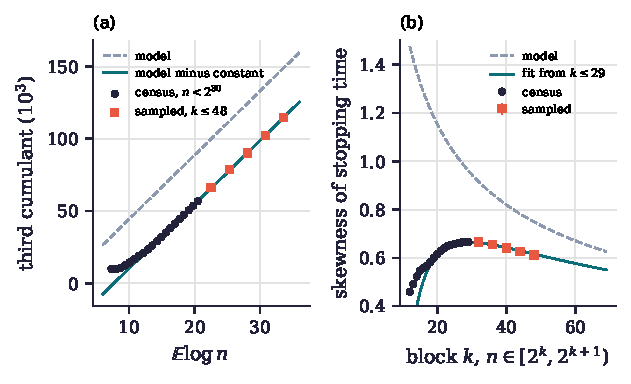
\includegraphics[width=\textwidth]{figures/ch16_o4.pdf}
\caption{The third cumulant of stopping times. (a) The third cumulant against
$\E\log n$: the census (dots), sampled blocks up to $k=48$ (squares), the
model line $A_3\,\E\log n$ (dashed) and the fit $a_3\,\E\log n-D_3$ (solid).
(b) Skewness: census, sampled blocks with two standard errors, the
prediction of the fit from $k\le29$, and the uncorrected model.}
\label{fig:ch16:o4}
\end{figure}

The variances agree to within $0.2$ percent, the third cumulants to within
$0.8$ percent, and the skewness to within two standard errors at every block,
while the uncorrected model is off by between $0.14$ and $0.25$. The skewness
peaks near $k=30$ and falls, as predicted: $0.640$ at $n\approx2^{40}$, a value
the model reaches only near $2^{66}$. Extrapolating, the skewness should be
$0.577$ at $2^{60}$ and $0.478$ at $2^{100}$, against model values $0.671$ and
$0.521$.

\paragraph{Status of O4.} The third cumulant is explained in the same sense as
the variance: the Bernoulli model is right about the slopes of the first three
cumulants to within a fraction of a percent, and the deficits behave as constants
contributed mostly by the finite system at the bottom of the orbit. The prediction
has been confirmed out of sample. What remains is a proof that the deficits
are bounded, which would require controlling the passage of the orbit from
the Terras horizon to the bottom, and that is the divergence half in
miniature. This also completes project P4 to the extent memory allows: the
sampled cumulants to $n\approx2^{49}$ show no departure from the fitted
constants.

\section{The exact convex rate of Switching MM}\label{sec:ch16:p11}

\Cref{conj:ch7b:tight} gave the worst case of $\smmdet$ on smooth convex
functions as $LR^2/((4+2\beta)N+2)$ for even $N$ and $\beta\le\beta_2$. We now
have a conjectured closed form for every $\beta<1$, and a proof for $N=2$ and $4$ on ranges of $\beta$ that contain the Collatz value.

\subsection{Two branches}

Write $D_N=(4+2\beta)N+2$ and $D'_N=4N-2+2(N-2)\beta$. The second quantity is
the same expression for the schedule that remains after the first long step:
$N-1$ steps, of which $N/2$ are unit steps and $N/2-1$ are long.

\begin{conjecture}[The exact convex rate of Switching MM, both branches]\label{conj:ch16:full}
For every even $N\ge2$ and every $0\le\beta<1$, the worst case of $\smmdet$ over
convex $L$ smooth functions with $\|x_0-x_*\|\le R$ is
\[
  \sup\bigl(f(x_N)-f_*\bigr)=LR^2\max\Bigl\{\frac1{D_N},\ \frac{\beta^2}{D'_N}\Bigr\}.
\]
The two branches cross at
\[
  \beta_N=\frac{\sqrt{9N^2-2N+1}-N-1}{2N},
\]
the positive root of $N\beta^2+(N+1)\beta-(2N-1)=0$, so that the main branch is
exact for all even $N$ exactly when $\beta\le\beta_2=(\sqrt{33}-3)/4=0.68614$.
\end{conjecture}

The crossing equation $\beta^2D_N=D'_N$ is the cubic
$2N\beta^3+(4N+2)\beta^2-2(N-2)\beta-(4N-2)=0$, which factors as
$(\beta+1)\bigl(2N\beta^2+(2N+2)\beta-(4N-2)\bigr)=0$; for $N=2$ it is the cubic
$2\beta^3+5\beta^2-3=(\beta+1)(2\beta^2+3\beta-3)$ of \cref{chap:threepoint}. The
thresholds are $\beta_2=0.6861$, $\beta_4=0.8381$, $\beta_6=0.8910$,
$\beta_8=0.9178$, $\beta_{10}=0.9341$, and $\beta_N\to1$. They agree with the
bisection values of \cref{chap:threepoint} to every digit computed, and
performance estimation agrees with the two branch formula to a relative error
below $2\times10^{-7}$ at $N=2,4,6,8,10$ and six values of $\beta$ on both sides
of each threshold, up to $\beta=0.99$ (script \texttt{ch16\_fullconj.py},
\cref{fig:ch16:smm}(a)).

\subsection{The lower bounds are attained by explicit functions}

\begin{proposition}[Two worst functions]\label{prop:ch16:lower}
For every even $N$ and $0\le\beta<1$ the supremum in \cref{conj:ch16:full} satisfies
\[
  \sup\bigl(f(x_N)-f_*\bigr)\ \ge\ LR^2\max\Bigl\{\frac1{D_N},\ \frac{\beta^2}{D'_N}\Bigr\}.
\]
\end{proposition}

\begin{proof}
Work in one dimension with $x_*=0$, $x_0=R$, and write $s_j\in\{1+\beta,1\}$ for the
step multipliers, so that a step from a point where the derivative is $c$
moves by $s_jc/L$.

For the first branch take the Huber function $f(x)=c|x|-c^2/(2L)$ for
$|x|\ge c/L$ and $f(x)=Lx^2/2$ otherwise, which is convex and $L$ smooth. As long
as the iterates stay in $x\ge c/L$ the derivative is $c$, so
$x_N=R-(W/2)c/L$ with $W=2\sum_js_j=(2+\beta)N$, and
$f(x_N)-f_*=cx_N-c^2/(2L)=cR-(W+1)c^2/(2L)$. The choice $c=LR/(W+1)$ gives
$LR^2/(2W+2)=LR^2/D_N$, and then $x_N=R(W+2)/(2(W+1))\ge c/L$, so every iterate
did stay in the linear region.

For the second branch take $f(x)=Lx^2/2$ for $x\ge-c/L$ and $f(x)=c|x|-c^2/(2L)$
for $x<-c/L$, again convex and $L$ smooth. The first step, of multiplier
$1+\beta$, starts in the quadratic region and lands at $x_1=R-(1+\beta)R=-\beta R$.
If $\beta R\ge c/L$ the remaining $N-1$ steps run in the linear region, and the
same computation with $R$ replaced by $\beta R$ and $W$ by
$W'=2\sum_{j\ge1}s_j=2N-2+(N-2)\beta$ gives $L\beta^2R^2/(2W'+2)=L\beta^2R^2/D'_N$, with
$c=L\beta R/(W'+1)\le L\beta R$ as required.
\end{proof}

The second function makes the meaning of the overshoot branch plain. A long
step on the quadratic part carries the iterate past the minimizer by a
fraction $\beta$ of the distance, and from there the remaining steps face the
method's own worst case, from distance $\beta R$. For small $\beta$ the overshoot is
harmless; beyond $\beta_N$ it is the worst thing that can happen.

\subsection{An explicit certificate}

The upper bound is the hard direction. Performance estimation solved with only
the inequalities between consecutive iterates and between each iterate and the
minimizer, the structure of the proof of Drori and Teboulle for gradient
descent, gives the same value as the full program (script
\texttt{ch16\_pep\_sparse.py}), so a certificate of that shape exists. Its
multipliers can be read off and have a closed form.

\begin{theorem}[An exact rate for two and four steps]\label{thm:ch16:cert}
Let $s_k=1+\beta$ for even $k$ and $s_k=1$ for odd $k$, let $x_{k+1}=x_k-(s_k/L)\nabla f(x_k)$ for $0\le k<N$ (for odd $k$ the point $x_k$ is the intermediate point $y$ of \cref{chap:threepoint}, and $x_N$ is the $N$th iterate of \smmdet), $W_k=2(s_0+\dots+s_k)$, and
\begin{gather*}
  \lambda_k=\frac{W_k}{D_N-W_k+2\beta\,[k\text{ even}]},\\
  \mu_0=\lambda_0,\qquad\mu_k=\lambda_k-\lambda_{k-1}\ (0<k<N),\qquad\mu_N=1-\lambda_{N-1}.
\end{gather*}
Multiply the interpolation inequality between iterates $k$ and $k+1$ by
$\lambda_k$ and the one between the minimizer and iterate $k$ by $\mu_k$, and sum.
The result is $f(x_N)-f_*\le LR^2/D_N-q$, where $q$ is a quadratic form in
$x_0-x_*$ and the gradients, and $q\ge0$ holds identically when
\begin{gather*}
  N=2\ \text{and}\ 0\le\beta\le b_2=0.64461,\qquad\text{or}\\
  N=4\ \text{and}\ 0\le\beta\le b_4=0.70438,
\end{gather*}
where $b_2$ and $b_4$ are the positive roots of $2\beta^4+11\beta^3+17\beta^2+\beta-11$
and $4\beta^4+21\beta^3+31\beta^2-\beta-23$. In these ranges, which contain the
Collatz value, \cref{conj:ch16:full} holds.
\end{theorem}

\begin{proof}
The multipliers are positive and increasing in $k$, since $W_k$ increases and the
denominator decreases, by $2$ from an odd $k-1$ to an even $k$ and by $2+2\beta$ from an
even $k-1$ to an odd $k$, and $\lambda_{N-1}=(2+\beta)N/((2+\beta)N+2)<1$, so all $\lambda_k$ and $\mu_k$ are nonnegative and $\sum_k\mu_k=1$. With these
weights the function values telescope to $f(x_N)-f_*$. The remaining quadratic
form has a matrix $S(\beta)$ of size $N+2$ in the basis $x_0-x_*,\nabla f(x_0),\dots,\nabla f(x_N)$,
computed symbolically in $\beta$ (script \texttt{ch16\_certificate.py}). It is
singular (its determinant vanishes identically), so it is positive semidefinite
if its leading principal minors of orders $1$ to $N+1$ are positive, since then its leading block of order $N+1$ is positive definite and the Schur complement of that block, a positive multiple of the determinant, is zero. For
$N=2$ these are, up to positive factors, $1$, $-(2\beta^2+3\beta-3)$ and
$-(2\beta^4+11\beta^3+17\beta^2+\beta-11)$, all positive on $[0,b_2)$, and $S(b_2)$ is positive semidefinite by continuity. For $N=4$ they
are, up to positive factors, $1$, $-(4\beta^2+5\beta-7)$, $-p(\beta)$,
$p(\beta)\,r(\beta)$ and $p(\beta)\,t(\beta)$, where $p=4\beta^4+21\beta^3+31\beta^2-\beta-23$,
$r=9\beta^4+42\beta^3+31\beta^2-84\beta-99$ and
$t=36\beta^6+312\beta^5+964\beta^4+1016\beta^3-722\beta^2-2280\beta-1287$; on $[0,b_4)$ the
polynomials $p$, $r$ and $t$ are all negative, so every minor is positive, and $S(b_4)$ is positive semidefinite by continuity.
Combined with \cref{prop:ch16:lower}, the bound is attained.
\end{proof}

Two features of the minors are worth recording. The second leading minor is
positive exactly below the true threshold: its factor $2\beta^2+3\beta-3$ for
$N=2$ and $4\beta^2+5\beta-7$ for $N=4$ is the crossing quadratic
$N\beta^2+(N+1)\beta-(2N-1)$. So the threshold of the conjecture is visible in the
certificate. The higher minors fail earlier, at $b_N<\beta_N$, which means that
these particular multipliers are optimal only in the lower part of the range
and a different certificate is needed near the threshold. Numerically the same
closed form multipliers give a positive semidefinite $S(\beta)$ for every even
$N\le20$ when $\beta$ is below a value that increases with $N$, from $0.6446$ at
$N=2$ to $0.7559$ at $N=20$, so the theorem very probably extends to all even
$N$ for $\beta\le b_2$, which includes $\beta=\lt-1$.

\paragraph{Status of P11.} The conjecture is now complete in closed form for
every $\beta<1$, both branches have rigorous lower bounds, and the upper bound is
proved for $N=2$ and $4$ on ranges containing the Collatz value. A proof for all
even $N$ along the lines of Drori and Teboulle, with the multipliers of
\cref{thm:ch16:cert}, needs the positivity of $S(\beta)$ in general, and a second
family of multipliers is needed between $b_N$ and $\beta_N$.

\section{Noise floors beyond quadratics}\label{sec:ch16:s2}

Problem S2 asks whether the noise bound $5/3$ of \cref{prop:ch7:bound} survives
beyond the quadratic model with isotropic noise, and project P5 asks for a test
on a real stochastic problem. We give a small extension and a test.

\begin{proposition}[Correlated noise]\label{prop:ch16:correlated}
On the quadratic of \cref{sec:ch7:model}, let the noise of the oracle have an
arbitrary covariance $Q$ instead of $\sigma^2I$, still independent from call to
call. Then for every step $\alpha\le1/L$ and every $0\le\beta<1$ the stationary excess loss
of $\smmdet$ is at most $5/3$ times that of gradient descent with the same step.
\end{proposition}

\begin{proof}
In the eigenbasis of $A$ all the methods act separately on each coordinate, so
the stationary covariance $C$ of the error satisfies
$\E[f-f_*]=\half\sum_i\lambda_iC_{ii}$, and $C_{ii}$ depends on the noise only through
the variance $Q_{ii}$ of its $i$th coordinate, linearly. By \cref{thm:smmvar}
applied to each coordinate, $C_{ii}^{\mathrm{SMM}}=r(a_i)\,C_{ii}^{\mathrm{GD}}$ with
$r\le5/3$ by \cref{prop:ch7:bound} and \cref{prop:ch7:uniform}. The ratio of
excess losses is therefore a weighted average of the $r(a_i)$, with nonnegative
weights $\lambda_iC_{ii}^{\mathrm{GD}}$.
\end{proof}

The correlations between coordinates, which make minibatch noise far from
isotropic, therefore do not matter on a quadratic. To see what the
nonlinearity does, we took the $\ell_2$ regularized multinomial logistic
regression on the digits data of scikit learn: $1797$ images, $64$ pixels and a
bias, ten classes, $650$ parameters, $\lambda=0.01$, so that $L=0.929$, $\mu=0.010$
and $\kappa=93$ at the minimizer (script \texttt{ch16\_s2\_softmax.py}). The linear
theory predicts the noise floor of each method from the Hessian $H$ at the
minimizer and the covariance $S$ of per sample gradients there, by solving the
discrete Lyapunov equation of the linearized dynamics with noise covariance
$S/b$ for minibatches of size $b$; for Switching MM the two step map is used.
The simulation runs each method on the true loss, from the minimizer, with step
$1/L$, for $20\,000$ iterations after a burn in, over six seeds.

\begin{table}[t]
\centering\small
\setlength{\tabcolsep}{4pt}
\caption{Noise floors $\E[f-f_*]$ on the digits problem, relative to gradient
descent, from the linear theory and from simulation, for minibatches of $16$
and $64$. Gradient descent itself: predicted $0.0660$ and $0.0165$, simulated
$0.0809$ and $0.0173$.}
\label{tab:ch16:s2}
\begin{tabular}{@{}lrrrr@{}}
\toprule
 & \multicolumn{2}{c}{$b=16$} & \multicolumn{2}{c}{$b=64$} \\
\cmidrule(lr){2-3}\cmidrule(l){4-5}
method & theory & simulation & theory & simulation \\
\midrule
Switching MM, $\beta=0.585$ & $1.094$ & $1.166$ & $1.094$ & $1.076$ \\
Nesterov, $\beta=0.585$ & $1.281$ & $2.049$ & $1.281$ & $1.428$ \\
Nesterov, $\beta=0.9$ & $2.198$ & $6.306$ & $2.198$ & $2.875$ \\
heavy ball, $\beta=0.9$ & $7.959$ & $21.77$ & $7.959$ & $10.60$ \\
\bottomrule
\end{tabular}
\end{table}

\Cref{tab:ch16:s2} and \cref{fig:ch16:smm}(b) give the result. At the
moderate noise level $b=64$ the linear theory predicts the absolute floor of
gradient descent to within five percent and that of Switching MM to within
three. At the heavy noise level $b=16$ the iterates wander far enough from the
minimizer for the curvature to change, every floor rises above the linear
prediction, and the rise is much larger for the momentum methods: every step
Nesterov at $\beta=0.9$ is six times worse than gradient descent instead of the
predicted two, and heavy ball twenty two times worse instead of eight.
Switching MM stays within $17$ percent of gradient descent at both noise
levels. The bound $5/3$ holds with room to spare on this nonquadratic problem,
and the nonlinearity widens the advantage of parity switching over every step
momentum rather than narrowing it.

\begin{figure}[t]
\centering
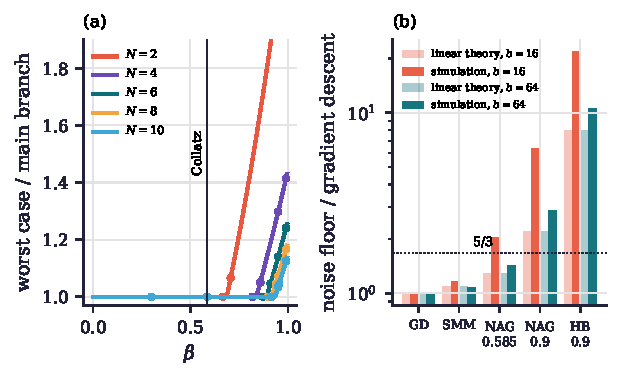
\includegraphics[width=\textwidth]{figures/ch16_smm.pdf}
\caption{(a) The worst case of Switching MM on smooth convex functions divided
by the main branch $LR^2/D_N$, from \cref{conj:ch16:full} (lines) and from
performance estimation (dots), for $N=2,\dots,10$. The overshoot branch takes over
at $\beta_N$. (b) Noise floors on the digits problem relative to gradient
descent: linear theory (pale) and simulation (solid) for minibatches of $16$
and $64$, with the bound $5/3$ dotted.}
\label{fig:ch16:smm}
\end{figure}

\paragraph{Status of S2 and P5.} Correlated noise is settled on quadratics.
The nonquadratic case remains open as a theorem, but on a real problem with
genuine minibatch noise the bound holds and the linear theory is accurate at
moderate noise. A test on deep networks, where the Hessian is not positive
definite, is the natural next step.

\section{Erd\H{o}s 125 to \texorpdfstring{$4^{17}$}{4 to the 17}}\label{sec:ch16:p7}

\Cref{sec:ch8:erdos} computed the density of $A+B$ exactly up to $4^{13}$, where
$A$ and $B$ are the integers whose base $3$ and base $4$ digits lie in $\{0,1\}$.
With a bit array and compiled loops (script \texttt{ch16\_erdos125.py}) the same
exact computation reaches $4^{17}=17\,179\,869\,184$, a range $256$ times
larger, in eleven minutes. It reproduces every value of
\cref{tab:ch8:erdos}. The new densities are $0.8760$, $0.7855$, $0.7936$ and
$0.8453$ at $4^{14}$ to $4^{17}$, and the minimum over $[10^4,4^{17}]$ is still
$0.763392$ at $3^{15}-1$.

The minima sit just below powers of $3$, and the computation shows what
controls their depth. Write $f_m$ for the fractional part of $m\log_43$, so
that $3^m=4^{\lfloor m\log_43\rfloor}\cdot4^{f_m}$. \Cref{tab:ch16:erdos} lists the
density at $3^m-1$ for $10\le m\le21$ against $f_m$.

\begin{table}[t]
\centering\small
\caption{Density of $A+B$ in $[0,3^m-1]$ against the fractional part $f_m$ of
$m\log_43$, sorted by $f_m$. Pairs of rows with close $f_m$ come from different
scales and have close densities.}
\label{tab:ch16:erdos}
\begin{tabular}{@{}rll@{\qquad}rll@{}}
\toprule
$m$ & $f_m$ & density & $m$ & $f_m$ & density \\
\midrule
$19$ & $0.057$ & $0.7924$ & $21$ & $0.642$ & $0.8312$ \\
$14$ & $0.095$ & $0.8147$ & $16$ & $0.680$ & $0.8312$ \\
$18$ & $0.265$ & $0.8813$ & $11$ & $0.717$ & $0.8372$ \\
$13$ & $0.302$ & $0.8742$ & $20$ & $0.850$ & $0.7679$ \\
$17$ & $0.472$ & $0.8590$ & $15$ & $0.887$ & $0.7634$ \\
$12$ & $0.510$ & $0.8583$ & $10$ & $0.925$ & $0.7785$ \\
\bottomrule
\end{tabular}
\end{table}

To within about $0.015$, the density at $3^m-1$ is a function of $f_m$ alone,
across a range of scales from $3^{10}$ to $3^{21}$
(\cref{fig:ch16:erdos}(a)). It is largest near $f_m\approx0.3$ and smallest near
$f_m\approx0.88$, where a power of $3$ lies a little below a power of $4$, at a
ratio $4^{f_m-1}\approx0.85$, and the gaps of $A$ and $B$ align, as described in
\cref{sec:ch8:erdos}. There is no visible drift with scale at fixed $f_m$: the pairs
$(15,20)$, $(12,17)$, $(13,18)$ and $(11,16,21)$ agree to within $0.007$. The
theorem of AlphaProof Nexus that the lower density is zero must therefore act
through approximations far better than any in range, such as
$3^{53}\approx4^{42}$ with $f_{53}=0.0015$, consistent with the windows its proof
uses.

\paragraph{Status of P7.} The computation is extended to $4^{17}$; the depth of
the minima is controlled by $f_m$ with no drift at fixed $f_m$ up to $3^{21}$. A
heuristic for the limiting profile as a function of $f_m$, and for the scale at
which it must begin to fall, would make the picture quantitative.

\section{Single orbits from \texorpdfstring{$2^{300000}$}{2 to the 300000}}\label{sec:ch16:p3}

Project P3 asks whether single orbits from much larger starting values show
any departure from independent sampling. We followed four Syracuse orbits
from random odd integers near $2^{100000}$, of about $241\,000$ steps each, and
one from near $2^{300000}$, of $723\,876$ steps, thirty times the scale of
\cref{sec:ch9:single} (script \texttt{ch16\_p3\_orbits.py}). Along each orbit we
tested four things, each against a null calibrated to the orbit's length.

\begin{itemize}[leftmargin=1.5em]
\item Residues modulo $3^a$ for $a=5,\dots,8$: the total variation distance of the
  empirical law from the stationary law $\pi_a$ of the induced chain is between
  $0.89$ and $1.06$ times the mean distance for independent samples from $\pi_a$
  of the same length (\cref{fig:ch16:erdos}(b)).
\item Consecutive residues modulo $3^4$: a $\chi^2$ statistic of the transition
  counts against the induced chain, restricted to cells with expected count at
  least $5$, lies within $1.7$ standard deviations of its distribution under
  the chain itself, simulated for the same length, on all five orbits.
\item Halving exponents: the means are $1.9992$, $1.9989$, $2.0034$, $2.0005$ and
  $1.9994$, against $2$, with $z$ scores between $-0.4$ and $1.2$; the
  autocorrelations at lags $1$ to $5$ are all below $0.0031$ in absolute value,
  against a standard error of $0.0020$, and $0.0012$ for the longest orbit.
\item Low binary digits modulo $2^{12}$: $\chi^2$ tests against the uniform law on
  odd classes give $p$ values $0.88$, $0.77$, $0.03$, $0.99$ and $0.05$, as
  expected of five independent tests.
\end{itemize}

\paragraph{Status of P3.} At thirty times the earlier scale, with moduli up to
$3^8$ and with joint and serial statistics, no statistic of a single orbit
departs from independent sampling. The evidence for trajectory mixing (O2)
is correspondingly stronger; the proof is as far away as before.

\begin{figure}[t]
\centering
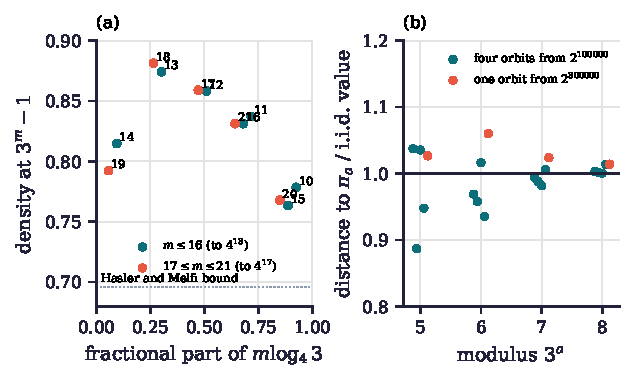
\includegraphics[width=\textwidth]{figures/ch16_erdos.pdf}
\caption{(a) Erd\H{o}s $125$: the density of $A+B$ at $3^m-1$ against the
fractional part of $m\log_43$, for $10\le m\le21$, labelled by $m$; the depth of
the minima depends on $f_m$ and not on the scale. (b) Single orbits: total
variation distance of the residues modulo $3^a$ from $\pi_a$, divided by its
mean under independent sampling, for four orbits from $2^{100000}$ and one from
$2^{300000}$.}
\label{fig:ch16:erdos}
\end{figure}

\section{Where the problems stand}\label{sec:ch16:status}

\Cref{tab:ch16:status} records the status of every problem of
\cref{chap:open} after this chapter and the rest of the book.

\begin{table}[t]
\centering\small
\setlength{\tabcolsep}{3pt}
\caption{Status of the open problems and projects.}
\label{tab:ch16:status}
\begin{tabular}{@{}l>{\raggedright\arraybackslash}p{0.80\textwidth}@{}}
\toprule
O1, O2 & open; P3 strengthens the evidence for O2 \\
O3, O3$'$ & open; \cref{chap:mmcollatz} rules out bounded depth \\
O4 & third cumulant explained and predicted out of sample (\cref{sec:ch16:o4}); boundedness of the deficits open \\
O5 & settled by \cref{prop:uimartingale}; no separate open problem \\
C1, C2, C3 & open \\
B1, B2, B3 & open \\
S1 & settled for the distance by \cref{thm:ch5b:rate}; the function gap for $\kappa<(1+\beta)/(1-\beta)$ open \\
S2 & open; on quadratics extended to any noise covariance (\cref{prop:ch16:correlated}); supported on a real problem \\
S3 & settled on quadratics by \cref{prop:ch7:pareto}; the choice of scale without $\mu$ open \\
S4 & open \\
P1, P2 & open \\
P3 & done to $2^{300000}$, no departure found \\
P4 & done to $n\approx2^{49}$ by sampling, consistent with constant deficits \\
P5 & done on one real problem; deep networks open \\
P6 & settled in the slow mode by \cref{thm:ch7:gainweight} \\
P7 & extended to $4^{17}$; minima controlled by $f_m$ \\
P8, P9, P10 & open \\
P11 & complete conjecture, both lower bounds, proof for $N=2$, $\beta\le0.6446$, and $N=4$, $\beta\le0.7043$ (\cref{sec:ch16:p11}) \\
\bottomrule
\end{tabular}
\end{table}

\section*{Notes}

The cumulants of first passage times of random walks, and the absence of a
third cumulant correction for symmetric steps, follow from Wald's identities
and are in Feller~\cite{feller1971} and Gut~\cite{gut1988}. The structure of the
certificate in \cref{thm:ch16:cert} follows Drori and Teboulle~\cite{drori2014};
the interpolation conditions are those of Taylor, Hendrickx and
Glineur~\cite{taylor2017}, and the Huber function is the classical worst case
for gradient descent. The digits data are distributed with scikit learn. The
Erd\H{o}s $125$ problem and its solution are discussed in \cref{sec:ch8:erdos},
with references there. All results in this chapter are new; the scripts are
listed in \cref{app:code}.

\section*{Exercises}

\begin{exercise}
For a random walk with increments $\pm\half\log3$ and drift $\mu<0$, use Wald's
identities to show that the third cumulant of the first passage time below
$-u$ grows like $3\sigma^4u/|\mu|^5$, and explain why a skewed step distribution
would add a term proportional to $\kappa_3$ of the step.
\end{exercise}

\begin{exercise}
Verify the factorization
$2N\beta^3+(4N+2)\beta^2-2(N-2)\beta-(4N-2)=(\beta+1)(2N\beta^2+(2N+2)\beta-(4N-2))$ and
show that $\beta_N\to1$ like $1-2/(3N)$.
\end{exercise}

\begin{exercise}
For the gradient method with an arbitrary step schedule $s_0,\dots,s_{N-1}$ in $(0,2)$, repeat the first half of the proof of
\cref{prop:ch16:lower} and show that the Huber function gives the lower bound $LR^2/(2W+2)$ with
$W=2\sum_js_j$. Check that for constant steps $s_j=1$ this is the bound
$LR^2/(4N+2)$ of Drori and Teboulle.
\end{exercise}

\begin{exercise}
Show that in the eigenbasis of $A$ the stationary covariance of gradient
descent with step $\alpha$ on the quadratic of \cref{prop:ch16:correlated} has
entries
\[
  C_{ij}=\frac{\alpha^2Q_{ij}}{1-(1-a_i)(1-a_j)},\qquad a_i=\alpha\lambda_i,
\]
and that only its diagonal enters the excess loss.
\end{exercise}
